\begin{titlepage}

	
\begin{center}
  

%\textsc{\LARGE  Eberhard Karls Universität Tübingen\\Mathematisch-Naturwissenschaftliche Fakultät\\ \institut\\
%Fachbereich \fachbereich}\\[4cm]


% Title
\newcommand{\HRule}{\rule{\linewidth}{0.5mm}}
\HRule \\[0.4cm]
\vspace{0.4cm}
{\large \bfseries \titel}\\[0.4cm]

\HRule \\[0.5cm]

\textsc{\large Exposé Bachelorarbeit}\\[0.3cm]

%\emph{Autor:}
\vorname \space \textsc {\name}  \\ 

%\emph{Matrikelnummer:}
\matrikelnr\\
[1.5cm]

\end{center}

A major problem in current research on neural networks, especially in classification and recognition tasks, is the size of training data sets needed, to yield accurate results. This is primarily due to way in which the network is trained to represent real world concepts. A neural network trains on many variations of the same concept, i.e 1000 pictures of a cat from different angles with separate light intensities. After this training process it can distinguish different categories with very high accuracy in many applications but reducing the number of variations would be beneficial to cut costs and training time. In the optimal case a reduction would go as far as one variant per concept. The network would then be able to see one representation of a concept and be able to identify others since it learns the essential features of this concept like a child that can be shown a picture of a horse and immediately has some idea of what other iterations of horses with varying features could look like.  

\\
%unhandliche interpretationen des feature space
The way in which we try to achieve this goal is by combining a generative model with a inverse classification approach. The process is structured in two steps. The first part is the training of a generative recurrent neural network (RNN) on a number of sequences representing letters. This is likely done by feeding the network a one-hot vector, representing a given class until it is able to produce this letter on its own. This has already been done experimentally to great success in (citation needed). The second part of the model is the inverse classification. Here, an undefined class, i.e. a vector full of zeros is presented as input and the picture to be classified given as the corresponding label. Likely the difference between generated output and label will be rather high. Gradients are then propagated through the network and a prediction for a class is given. This prediction is put into the network again and the process is repeated until the class vector converges. In the optimal case it again is a one-hot vector representing the letter of the image that we wanted to classify. Importantly the networks weights are not changed in the second step but only the current representation of the class vector. The concept of inverse classification as already been shown to successfully execute goal-directed policy inference online \cite{RocketballOtte2017}. The whole model can be seen in figure \ref{model_figure}.\\
\begin{figure}
	\begin{minipage}[c]{0.67\textwidth}
		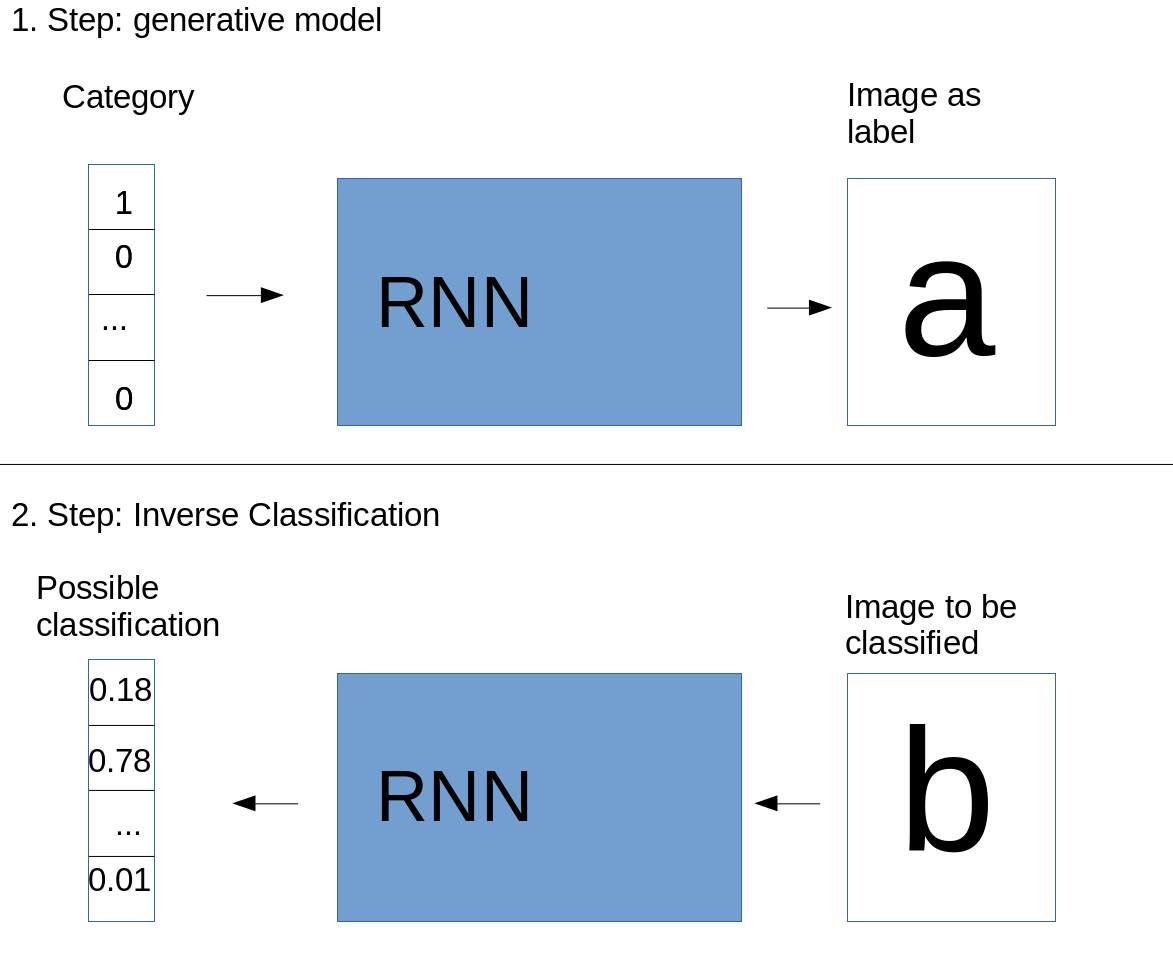
\includegraphics[width=\textwidth]{model_figure.png}
	\end{minipage}\hfill
	\begin{minipage}[c]{0.33\textwidth}
			\caption{\small{Top: A generative model is trained by input of a one-hot vector and showing sequences representing handwritten letters as labels. \\
					Bottom: Inverse classification process: class is guessed, compared to actual sequence and then adapted. After some iterations class should be converging to the real letter.}}
			\label{model_figure}
	\end{minipage}
\end{figure}
\begin{figure}[!h]
	
	

\end{figure}

A similar approach, combining a generative model with a classification network, is taken in variational autoencoders, published in \autocite{VAE2017}. This work tries to extent autoencoders in two ways. Firstly, the generative and the classifying model are the same network, while in autoencoders two different models are used. Having the same models for both tasks might lead to more meaningful internal representations of concepts such as features of letters. Secondly the latent space for autoencoders is generated during the training process and therefore not naturally interpretable by humans. In our case the latent space is essentially the class distribution for the letters, hopefully increasing interpretability of the classification results. \\

If the RNN is unable to fulfill this task, a second approach with variational autoencoders might be tried. 

 




\vspace{8pt}

Time-table: 
\vspace{-8pt}
\begin{itemize}
	\item 1. month: Find suitable datasets, implement RNN read related work
	\item 2. month: Implement inverse classification, optimize RNN and run tests
	\item 3. month: If possible implement a variational autoencoder and combine with inverse classification
	\item 4. month: Write down results of the experiments and compare the results to expectations and similar work
\end{itemize}
%
\printbibliography
\end{titlepage}
